\section{LNET: Lustre Networking}
\label{sec:lnet}

LNET is a message passing API, originated from Sandia Portals.  Although there
are commonalities between the two, they are not the same thing. We will cover the
Lustre LNET without delving into the differences between the two. 

\subsection{Core Concepts}

First, we need to clarify some terminology used throughout the rest of the
section, in particular, the process id, matching entry, matching bits, and
memory descriptor.

\begin{figure}[htb]
\centering
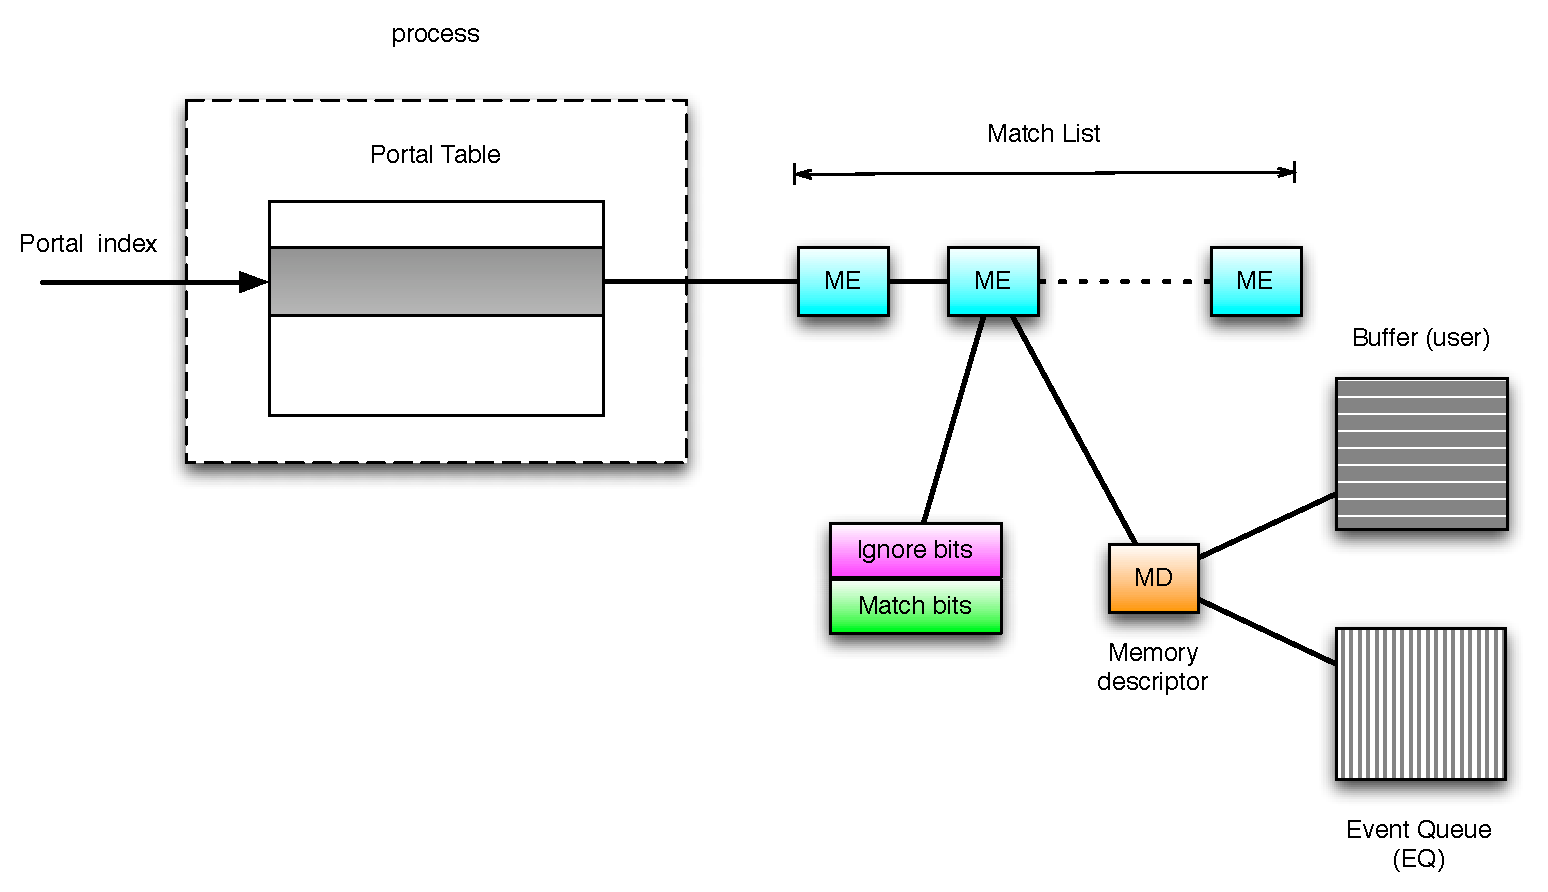
\includegraphics[width=5in]{img/lustre_portal_address}
\label{fig:lustre_portal_address}
\caption{Illustration of Lustre LNET addressing scheme.}
\end{figure}

\subsubsection*{LNET Process Id}

LNET identifies its peers using the LNET process id, defined as follows:

\begin{Verbatim}
typedef struct {
    lnet_nid_t  nid;
    lnet_pid    pid;
} lnet_process_id_t;
\end{Verbatim}

The \url{nid} identifies the id of the node, and \url{pid} identifies
the process on the node. For example, in the case of socket LND (and
for all currently existing LNET LNDs), there is only one instance of LNET
running in the kernel space; the process id therefore uses a reserved ID
(12345) to identify itself.

\subsubsection*{ME: Matching Entry}

A \textit{portal} is composed of a list of match entries (ME). Each ME can be
associated with a buffer, which is described by a memory descriptor (MD). ME
itself defines match bits and ignore bits, which are 64-bit identifiers that
are used to decide if the incoming message can use the associated buffer space.
Figure \ref{fig:lustre_portal_address} illustrates the Lustre LNET addressing
scheme.


\begin{Verbatim}
typedef struct lnet_me {
        struct list_head   me_list;
        lnet_libhandle_t   me_lh;
        lnet_process_id_t  me_match_id;
        unsigned int       me_portal;
        __u64              me_match_bits;
        __u64              me_ignore_bits;
        lnet_unlink_t      me_unlink;
        struct lnet_libmd *me_md;
} lnet_me_t;
\end{Verbatim}

All MEs associated with the portal are linked by the \url{me_list}.  The
\url{me_match_id} defines which remote LNET peer(s) are allowed to access this
ME, and it can be a wildcard that allows open access.

\subsubsection*{MD: Memory Descriptor}

Following the creation of an MD by the upper layer, the LNET layer uses
the~\url{struct lnet_md_t} to reference the MD. The LNET internal
representation is described by \url{struct lnet_libmd_t}.  Per our
understanding, the purpose is to make \url{lnet_libmd_t} opaque to the client
so that they cannot interfere with LNET internal states. They share some of the
common fields, but LNET maintains more states for internal housekeeping.

\begin{Verbatim}
typedef struct {
        void             *start;
        unsigned int     length;
        int              threshold;
        int              max_size;
        unsigned int     options;
        void             *user_ptr;
        lnet_handle_eq_t eq_handle;
} lnet_md_t;
\end{Verbatim}

If a memory buffer described by MD is contiguous, then the address of
\url{start} points to the begining of the memory. Otherwise, it points to the
start of some I/O vectors.  There can be two kinds of I/O vectors: if the
memory is already mapped to virtual memory, it is described by \url{struct
iovec}; otherwise, it is described by \url{lnet_kiov_t}, which may or may not be
mapped to virtual memory, and by definition, it is just a memory page.  MD
options (\url{options}) identifies the type of I/O vectors. It is either
\url{LNET_MD_IOVEC} or \url{LNET_MD_KIOV}. Also, if the MD is describing a
non-contiguous memory, \url{length} then describes the number of entries in the
array.

As mentioned above, \url{struct lnet_libmd_t} is used by LNET internal to
describe the MD along with some other bookkeeping fields:

\begin{Verbatim}
typedef struct lnet_libmd {
    struct list_head    md_list;
    lnet_libhandle_t    md_lh;
    lnet_me_t           *md_me;
    unsigned int        md_length;
    unsigned int        md_offset;
    unsigned int        md_niov;
    union {
        struct iovec    iov[LNET_MAX_IOV];
        lnet_kiov_t     kiov[LNET_MAX_IOV];
    } md_iov;
    ...
}
\end{Verbatim}

It should be obvious that \url{md_me} is the address of the ME entry this MD is
associated with, and it can be \url{NULL}. The \url{md_length} is the total
number of bytes of all segments this MD describes, and \url{md_offset} is the
number of bytes to skip. For a noncontiguous memory, think of it as all being
combined into a virtual contiguous array and you have a logical offset into it.
The \url{md_niov} is the number of valid entries of the I/O vectors described
by either \url{iov} or \url{kiov} in the union struct. \url{md_list} is a
hashtable with handle (\url{md_lh}) as key to locate an MD.

\subsubsection*{Example Use of Offset}

Upon initialization, the server will \textit{post} request buffers (for the request
portal); the buffer is to accommodate incoming client requests. We further
assume that the request buffer is 4KB in size and each request should be 1KB at
most. When the first message comes, the offset is increased to 1KB, and with the
second message, the offset is set to 2KB and so on. So essentially, the offset
is used to keep track of the write position to fend off an overwrite, and this is
the default case. Another case where offset is being used differently will be
described after we talk about MD options.

\subsubsection*{MD Options}

If the MD has the \url{LNET_MD_MANAGE_REMOTE} flag set, then the client can
indicate the offset into the MD for the GET or PUT operations. In the follow-on
API discussion, we describe the offset parameter in the GET and PUT API.
We describe two use cases here: 

\begin{itemize}

\item The router posts a buffer containing the nids for interested clients to read,
with \url{LNET_MD_MANAGE_REMOTE} and \url{LNET_MD_OP_GET} flags set. All clients
will get the buffer with offset as zero since they will get a complete list of nids
on the router.

\item For the case of an early server reply when adaptive timeout is in use,
the client posts one reply buffer before sending out the request. The server first
responds with an early reply with the offset set to zero. This means ``I got your
request, now wait patiently." Later, the server sends the actual reply to the
same buffer with the proper offset.  

\end{itemize}

Another type of attribute associated with the MD defines the operations
allowed on the MD. For example, if the MD only has a get flag
\url{LNET_MD_OP_GET}, then writing into this MD is not allowed. This is
equivalent to the read-only case. And \url{LNET_MD_OP_PUT} means the MD only
allows for a PUT operation, but without the GET flags, it becomes a write-only. 

There are two flags dealing with the case where an incoming message is bigger
than the current MD buffer. The \url{LNET_MD_TRUNCATE} allows a save but
truncates the message. This is useful when the client does not care about the
content of the reply. As an example, let's assume a client pings the router to
see if it is alive. The router replies with a list of its nids. The client does
not care about the contents and does not interpret those nids, so a small
buffer with a truncate flag is just fine.  The second flag is
\url{LNET_MD_MAX_SIZE}, which tells LNET to drop the message if the incoming
message is beyond the allowed size.

\subsubsection*{Event Queue}

Each MD has an event queue to which events are delivered. Each event queue can use 
callbacks or it can be polled.

\subsection{Portal RPC: A Client of LNET}

Portal RPC by design has multiple portals for each service defined, and these
are \textit{request}, \textit{reply}, and \textit{bulk} portals.  We use an
example to illustrate the point. Say a client wants to read ten blocks of data
from the server. It first sends an RPC request to the server telling that it
wants to read ten blocks and it is prepared for the bulk transfer (meaning the
bulk buffer is ready). Then, the server initiates the bulk transfer. When the
server has completed the transfer, it notifies the client by sending a reply.
Looking at this data flow, it is clear that the client needs to prepare two
buffers: one is associated with \textbf{bulk Portal} for bulk RPC, the other
one is associated with \textbf{reply Portal}.

This is just how Lustre makes use of Portal RPC. It uses two portals in the
above scenario because Portal RPC uses the same ME match bits for both.
However, it is fine to have two buffers posted using the same portal as long as
their ME matching bits are different.

\subsubsection*{Get and Put Confusion}

\begin{itemize}

\item Most of the time, a client issues \url{LNetPut} to request something from
the server or to request that something be sent to the server. Then the server will use
\url{LNetPut} to send a reply back to the client or \url{LNetGet} to read
something from the client as in bulk transfer.

\item The one case that a client will issue \url{LNetGet} is the router pinger;
the client will recieve a list of NIDs from a well-known server portal as a way
of verifing that the router is alive.

\end{itemize}

\subsubsection*{Router In the Middle}

We will use LNET PUT as an example to explain this scenario. Let's assume the
client, $C$, has some payload to send to a server $S$, as the final destination
through a router in the middle, $R$, as shown in Figure~\ref{fig:crs}. LNET
takes the payload and appends the PUT header with information such as final
server NID, match bits, offset, etc. This is now a complete LNET message. Then
the LNET passes this message on to the LND layer, along with the router NID. LND
puts this message on the wire, and this message will be
transmitted to $R$. 

The router LND layer receives this message and passes onto the router LNET
layer. Two pieces of information are needed from the PUT header in the message.
One is the size of the message so that router can allocate (or pre-allocate)
space to store the incoming message, noted that this space has nothing to do
with the MD we discussed before, it is just a piece of buffer. The second piece
of information is the destination NID. After the message is completely
recieved, router LNET will pass this message along with destination NID to
proper LND (it can be a different LND if this is heterogeneous routing
environment) to send it on the wire.

\begin{figure}[hbt]
\centering
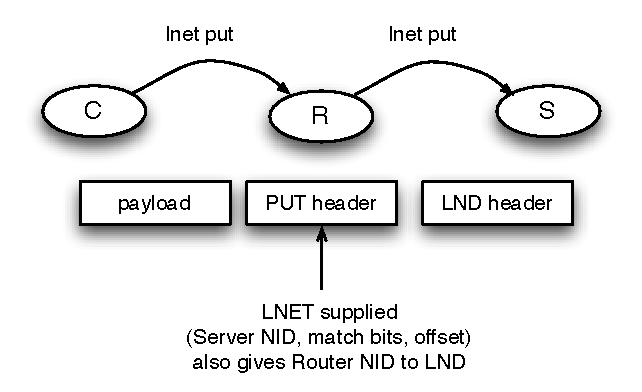
\includegraphics[width=3.5in]{img/lnet_crs}
\caption{The illustration of LNET PUT with a router in the middle scenario.}
\label{fig:crs}
\end{figure}


\subsubsection{Round 1: Client Server Interactions}

Assume that a server wants to expose a buffer to its client; below are the
steps happening on both sides, described briefly:

\begin{enumerate}

\item Server attaches the ME and MD and makes them part of some known
portal.

\item Server makes sure that the MD option is set correctly: get-only, for remote management
in this case. Now the server side is ready.

\item Client prepares the local ME and local MD for the reply if so requested.

\item Client invokes the LNET GET, with peer address, portal, match bits, etc.

\item Server receives the GET message, checks its validity (correct portal, correct
match bits, correct operation on the MD).

\item Server invokes the callback registered on the MD to notify the upper
layer. In the case of the router ping scenario we described earlier, once the
buffer is posted, the server at the upper layer may not be interested in client
requests, so this callback could just be NULL.

\item Server sends a reply message back to the client. Note that this
reply is \textbf{\textit{not}} a LNET PUT.

\end{enumerate}


\subsubsection{Round 2: More details}

\begin{enumerate}

\item Server posts a request buffer by \url{ptlrpc_register_rqbd()}. The \url{_rqbd}
is an abbrevation for request buffer descriptor, defined by the
\url{struct ptlrpc_request_buffer_desc}. It holds enough information for
creating the ME and MD. Since this is a server buffer that is to serve the request,
the matching id, as well as all important ME, MD creation is as follows:

\begin{Verbatim}
struct ptlrpc_service *service = rqbd->rqbd->rqbd_service;
static lnet_process_id_t match_id = {LNET_NID_ANY, LNET_PID_ANY};
rc = LNetMEAttach(service->srv_req_portal, match_id, 0, ~0,
                    LNET_UNLINK,LNET_INS_AFTER, &me_h);
rc = LNetMDAttach(me_h, md, LNET_UNLINK, &rqbd->rqbd_md_h);
\end{Verbatim}

\url{LNET_UNLINK} indicates this ME should be unlinked when the MD associated
with it is unlinked, and \url{LNET_INS_AFTER} means that the new ME should be
appended to the existing list of MEs. The \url{me_h} and \url{md} are defined as
\url{lnet_handle_me_t} and \url{lnet_md_t}, respectively.

\item Client sends an RPC by \url{ptl_send_rpc()}, and this function takes
\url{struct ptlrpc_request *request} as an input parameter and \textit{may}
perform the following operations:

  \begin{itemize}

  \item Client posts bulk buffer by \url{ptlrpc_register_bulk()}. This is performed
  when the bulk buffer is not NULL in the reqeust:

  \begin{Verbatim}
    if (request->rq_bulk != NULL) {
        rc = ptlrpc_register_bulk(request);
        ...
   \end{Verbatim}

  \item Client posts reply buffer by \url{LNetMEAttach()} and \url{LNetMDAttach()}.
  This operation is performed when a reply is expected (the input parameter
  \url{noreply} is set to 0).

  \item Client sends request: 
  \begin{Verbatim}
       rc = ptl_send_buf(&request->rq_req_md_h,
                          request->rq_reqmsg, request->rq_reqlen,
                          LNET_NOACK_REQ, &request->rq_req_cbid,
                          connection,
                          request->rq_request_portal,
                          request->rq_xid, 0);
  \end{Verbatim}

  \end{itemize}

\item Server handles incoming RPC by \url{request_in_callback()} defined in
\url{events.c}. This can incur two further actions:

  \begin{itemize}

  \item bulk transfer: \url{ptlrpc_start_bulk_transfer()},

  \item send reply: \url{ptlrpc_reply()}.

  \end{itemize}

\item Once the bulk transfer has been written, read, or replied to, there could be
more callback invoked such as \url{client_bulk_callback()} and
\url{reply_in_callback()}.

\end{enumerate}

\subsection{LNET API}

\subsubsection*{Naming Conventions}

Function names starting with \url{LNet} are external APIs for the upper
layers. All other functions using lower cases are internal to LNET.  Within
LNET, LND has two sets of APIs. If it starts with \url{lnd}, then it is the
API for LNET layer to call down or if it starts with \url{lnet}, then it is
for LND to call up into LNET, as illustrated in the figure below. Note that it
is confusing to use LNET to describe both as the whole network subsystem and
as a particular layer paramount to LND, but that seems the way it is being
used.

LNET compiles for both kernel space and user space. If a file is prefixed with
\url{liblnet}, it is meant for user space; otherwise, it is for kernel
space. Files under lnet/lnet are compiled twice, and those under
\url{lnet/klnds} and \url{lnet/ulnds} are compiled only once.


\begin{Verbatim}
        LNetPut      LNetGet
           |           |
      +--------------------+
      |        LNET        |
      +--------------------+               
      |     |          |   |
      |     v          v   |
      | lnd_send   lnd_recv|
      |                    |
      |        LND         |
      +--------------------+
\end{Verbatim}

\subsubsection*{Initialization and Teardown}

\url{int LNetInit(void)} and \url{int LNetFini(void)} are two APIs for
setting up and tearing down LNET connections.


\subsubsection*{Memory-Oriented Communication Semantics}

The following API has been annotated with comments:

\begin{Verbatim}
int LNetGet(
    lnet_nid_t        self,
    lnet_handle_md_t  md_in,        /* local MD to hold requested data */
    lnet_process_id_t target_in,    /* target process id */
    unsigned int      portal_in,    /* target portal index */
    __u64             match_bits_in,/* match bits used on target process */ 
    unsigned int      offset_in);   /* offset into remote MD */
\end{Verbatim}

This function initiates the remote read operation.  Note that \url{offset_in}
is only used when a target memory descriptor has the \url{LNET_MD_MANAGE_REMOTE}
flag set. It is the same for the PUT operation.

\begin{Verbatim}
int LNetPut(
    lnet_nid_t        self,
    lnet_handle_md_t  md_in,        /* local MD holding data to be sent */ 
    lnet_ack_req_t    ack_req_in,   /* flag to request Ack event */
    lnet_process_id_t target_in,    /* target process id */
    unsigned int      portal_in,    /* target portal index */
    __u64             match_bits_in,/* match bits for target process */
    unsigned int      offset_in,    /* offset into remote MD */
    __u64             hdr_data_in); /* 64-bit user data */
\end{Verbatim}

This function sends data asynchronously. The \url{self} specifies the
source NID to use and hence the outgoing NI (network interface).  If
\url{LNET_NID_ANY} is given, LNet will choose source NID and NI by itself,
based on destination NID and routing table.  Note that acknowledgments are
sent only when they are requested by the initiating process \textit{and} the
local MD has event queue \textit{and} remote MD enables them.

\subsubsection*{Match Entry Management}

\begin{Verbatim}
int
LNetMEAttach(unsigned int portal,
    lnet_process_id_t match_id, 
    __u64 match_bits, __u64 ignore_bits,
    lnet_unlink_t unlink, lnet_ins_pos_t pos, 
    lnet_handle_me_t *handle)
\end{Verbatim}

This function creates a new ME. The first parameter indicates which local
portal this ME should be associated with, and the next parameter indicates the
remote process id (or remote peer) allowed to access this ME. The rest are
match bits and ignore bits. Each portal RPC has a unique transaction id, so the
portal RPC uses this transaction id as the match bits for the reply. The
transaction id will be sent over to the remote peer, and the remote peer will
use this transaction id as the match bits in its reply buffer. The last
parameter is an ME pointer; if the call succeeds, it returns a handler.

\begin{Verbatim}
int LNetMDAttach(
    lnet_handle_me_t meh, /* ME to be associated with */
    lnet_md_t umd,        /* user-visible part of the MD */
    lnet_unlink_t unlink, /* if MD is unlinked when it is not active */
    lnet_handle_md_t *handle)
\end{Verbatim}

This function is used to create an MD and attach it to an ME. An error returns if
the ME already has an MD associated with it. \url{umd} comes from LNET client
(Portal RPC or LNET self-test for now), and it specifies parameters for the
to-be-created MD object, to which a handle will be returned in the
\url{lnet_handl_md_t *handle}.

\begin{Verbatim}
int LNetMDBind(
    lnet_md_t umd, 
    lnet_unlink_t unlink, 
    lnet_handle_md_t *handle)
\end{Verbatim}

This function creates a \textit{standalone} memory descriptor, i.e., an
MD that is not attached to an ME.

\subsection{LNET/LND Semantics and API}

LNET is connectionless, asynchronous, and unreliable. However, most LNDs are
reliable and connection-oriented such that they need to establish a connection
before they can talk to their peers. A LNET message has a payload restriction
of 1MB, \textit{and} the maximum number of segments cannot exceed 256.
Furthermore, LNET does not fragment or assemble fragments. It's assumed that
the upper layer never gives LNET a bigger payload than 1MB.  There are several
reasons for this limitation---for example the pre-set limit makes buffer
management easier and some low-level driver has a limit on the number of
scatter-gather buffers, such as 256. Also, an upper layer such as Portal RPC
can fragment data more easily if buffers are posted in pages. The downside to
this limitation is that if there is ever a network technology that supports an
MTU more than 1MB, then LNET might not be able to make full use of its
bandwidth.  \footnote{MTU is used for allocating the network bandwidth fairly.
For example, bigger MTU values might cause a malicious client to consume
the network bandwidth unfairly, while other clients might be starving.}

LND can have multiple instances---for example, in the cases where you have more
than one IB interface. Each interface is represented by a network interface
type defined by \url{lnet_ni_t}. One of the fields defined in that structure
is \url{lnd_t}---a method table callable on this particular LND type.

\subsubsection{API Summary}

LND APIs are the interface between LNET and its underlying network drivers. As
mentioned before, there are two sets of LND APIs. The first set is what LNET
expects LNDs to implement. For example, LNET expects to call LND methods to
send and receive messages. 

\begin{itemize}

\item \url{lnd_startup()}, \url{lnd_shutdown()}: These functions are called
per interface, whenever LNET wants to bring up or shut down the interfaces.

\item \url{lnd_notify()}: This is optional.

\item \url{lnd_accept()}: This is optional.

\item \url{lnd_send()}, \url{lnd_recv()}, \url{lnd_eager_recv()}: Sends
outgoing messages and receives incoming messages.

\item \url{lnd_ctl()}: This call is optional. It passes user space \url{ioctl}
commands to LND. LNET supports many ioctls through a special device file; some
are directly handled by LNET (for example, adding a route) and others must be
passed onto LND to handle.

\end{itemize}

The other set of APIs are LNET functions exported for LNDs to use:

\begin{itemize}

\item \url{lnet_register_lnd()} and \url{lnet_unregister_lnd()}: Each LND
driver calls this function to register a new LND type.

\item \url{lnet_notify()}: If a peer goes down, this function is called to
notify LNET.

\item \url{lnet_parse()}: For each new message received, LND calls this
function to let LNET know that a message has just arrived, so that LNET can
parse the message and check into it.

\item \url{lnet_finalize()}: This is called by LND on both incoming and
outgoing messages. When a message is sent, this call by LND allows LNET to
generate an event to tell that the message has been sent. For an incoming message,
this calls indicates the payload of the incoming message that has been
completely received.

\end{itemize}

\subsection{LNET Startup and Data Transfer} 

Brief notes on LNET code organizations:

\begin{Verbatim}
lnet/ulnds      /* LND in user space, */
lnet/klnds      /* LND in kernel space */
lnet/lnet       /* LNET layer */
\end{Verbatim}

Apparently, there is not much code sharing between the kernel LND and the user space
LND. Only Portals network and TCP network have an user space LND for that
reason. In the kernel space, \url{ptllnd} \footnote{For Cray SeaStar system.},
\url{o2iblnd}, and \url{socklnd} are probably the most important ones to know. 

\subsubsection{Startup}

\url{lnet_startup_lndnis()} is invoked when LNET gets initialized.

\begin{enumerate}

\item Calls on \url{lnet_parse_networks()} to parse module parameters 
provided by the user. Afterwards, LNET gets a list of network interfaces to bring
up.

\item Iterates each of the interfaces acquired above. First it tries to locate
the lnd instance represented by \url{lnd_t}. Upon finding it, it invokes the
\url{lnd_startup()}. We will look at each step in more detail.

\item Within the loop, it first looks for the driver by network type:

\begin{Verbatim}
lnd = lnet_find_lnd_by_type(lnd_type);
\end{Verbatim}

If a driver is not found, then it could be that the driver has not been loaded
yet, so it will try to load the module and then retry to locate the driver:

\begin{Verbatim}
rc = request_module(libcfs_lnd2modname(lnd_type));
\end{Verbatim}

After the driver is loaded, during its module initialization, it registers with
LNET, allowing the driver to be located later on.

\item After the driver for the network interface is located, then we can
\textit{bind} this driver to the interface and invoke the driver's startup
method:

\begin{Verbatim}
ni->ni_lnd = lnd;
rc = (lnd->lnd_startup)(ni);
\end{Verbatim}

\end{enumerate}

Now we will explain a specific LND module, socket LND. In particular, we look
into \url{ksocknal_startup()}.

\begin{enumerate}

\item If the function is being called for the first time, then it invokes
\url{ksocknal_base_startup()} to do some one-time initialization, for
example, creating the data structure shared by all interfaces.

\item Finds out which Ethernet interface to use for this network. It can be
user-specified or it can search for the first non-loopback interface in the
system.  Once located, it initializes the data structure for this interface.
The nid is generated by:

\begin{Verbatim}
ni->ni_nid = LNET_MKNID(LNET_NIDNET(ni->ni->nid),
    net->ksnn_interfaces[0].ksni_ipaddr);
\end{Verbatim}

\end{enumerate}

After LNET is initialized, a user can send or receive data on this interface.

\subsubsection{LNET Send}

We describe the general flow of the send path, starting from \url{LNetPut}
down to the LND layer.

\begin{enumerate}

\item First, the LNET message descriptor is allocated, \url{msg}, defined by
\url{struct lnet_msg_t}. This message descriptor will be passed on to LND. In
particular, there is a field within defined as \url{lnet_hdr_t msg_hdr} (the
message header) which will eventually be a part of the on-the-wire message.

\begin{Verbatim}
msg = lnet_msg_alloc();
\end{Verbatim}

\item LNET MD handle is converted from the incoming parameter to a real MD
structure, which will hold the payload:

\begin{Verbatim}
md = lnet_handle2md(&mdh);
\end{Verbatim}

\item The MD is associated with the message:

\begin{Verbatim}
lnet_commit_md(md, msg);
\end{Verbatim}

\item Message details are filled in. These details can be the type of message (PUT or GET),
match bits, portal index, offset, and user-supplied data, if any.

\begin{Verbatim}
lnet_prep_send(msg, LNET_MSG_PUT, target, 0, md->md_length);
msg->msg_hdr.msg.put.match_bits = cpu_to_le64(match_bits);
msg->msg_hdr.msg.put.ptl_index = cpu_to_le32(portal);
...
\end{Verbatim}

\item The event information is filled in as given below.

\begin{Verbatim}
msg->msg_ev.type = LNET_EVENT_SEND;
msg->msg_ev.initiator.nid = LNET_NID_ANY;
msg->msg.ev.initiator.pid = the_lnet.ln_pid;
...
\end{Verbatim}

\item Finally, lnet send function (not LND send) is invoked as below.

\begin{Verbatim}
rc = lnet_send(self, msg);
\end{Verbatim}

\item This send function needs to locate the interface to use. If the
destination is local, then it resolves to the directly attached interface. If
the destination is remote, then it resolves the interface to a router from the
routing table.  The result of this search is \url{lp}, defined by \url{struct
lnet_peer_t}, representing the best choice of a peer. This peer can be either
the interface for the router or the interface for the final destination as
below.

\begin{Verbatim}
msg->msg_txpeer = lp;
\end{Verbatim}

\item Next, \url{lnet_post_send_locked()} is called for credit checking.
Suppose you are only allowed to send $x$ number of concurrent messages to the
peer. If you exceed this credit threshold, the message will be queued until
more credits are available.

\item If credit checking passed, then:

\begin{Verbatim}
if (rc==0)
    lnet_ni_send(src_ni, msg);
\end{Verbatim}

This send function invokes LND send for further sending:

\begin{Verbatim}
rc = (ni->ni_lnd->lnd_send)(ni, priv, msg);
\end{Verbatim}

At some later point, after LND finishes sending the message,
\url{lnet_finalize()} will be called to notify the LNET layer that the message
is sent. However, let's continue down the path of sending data. Let's assume it
is an IP network; then socket LND send, more specifically,
\url{ksocknal_send()} will be called. 

\item Remember that socket LND is connection based, so when you want to send
something, first you need to locate the peer, then you have to check if a
connection has been established. If there is one, you just queue the \url{tx}
to the connection.

\begin{Verbatim}
if (peer!=NULL) {
    if (ksocknal_find_connectable_route_locked(peer) == NULL) {
        conn = ksocknal_find_conn_locked(tx->tx_lnetmsg->msg_len, peer);
        if (conn != NULL) {
            ksocknal_queue_tx_locked(tx,conn);
            ...
 }
\end{Verbatim}

So eventually, the message queued will be sent on the socket connection
through the kernel socket API. 

\item If there is no connection yet, then we queue the message to peer first,
so that when a new connection is established, we can move the message from the 
peer's queue to the connection's queue to be sent out.

The message format sent on the wire has the following layout, briefly:

\begin{Verbatim}
 +--------------+-----------+-----------------+-------------+-----------+
 | TCP, IP, and | sock LND  | LNET msg type   | LNET common |  payload  |
 | MAC header   | header    | specific header | header      | (from MD) |
 +--------------+-----------+-----------------+-------------+-----------+
\end{Verbatim}

\item There are two ways (APIs) to send a message from socket LND: If the
message is small, normal send will put the message into a kernel socket
buffer (each socket has a send buffer). This is \textit{not} a zero-copy
transfer.  Alternatively, you could send this buffer directly onto the network
without making a copy first (zero copy transfer). However, zero-copy has its
own overhead, so Lustre only utilizes this path for large messages.

\end{enumerate}


\subsubsection{LNET Receive}

On the receiving end, assuming that we are using socket LND, 
\url{ksocknal_process_receive()} is the entry function for receiving. The
general steps are given here.

\begin{enumerate}

\item LND starts to receive the new message. At first, it only receives up to LNET
message header because it doesn't know where to put the payload yet, only LNET
layer has the information on the destination MD.

For this reason, LND gives LNET header to \url{lnet_parse()}. This function
LNET layer will look into the header and identify the portal, offsets,
match bits, source NID, source PID, etc. LNET can either reject the message (for
example, malformed) or accept it.

\item If proper MD is located, LNET (from \url{lnet_parse()} calls another
LND API,  \url{lnd_recv()}. Now the payload from the socket kernel buffer is copied
over to the destination MD. In the case of socket LND, this is one kernel
memory-to-memory copy.
 

\item LNET calls \url{lnd_eager_recv()} immediately if it will call \url{lnd_recv()}
sometime later.

\item After LNET calls \url{lnd_recv()}, LND starts receiving the payload
(either by memory-to-memory copy or RDMA) and LND should call
\url{lnet_finalize()} within a finite time. LND could use RDMA for data
transfer at this point if it is available.

\end{enumerate}

Also note that TCP can perform fragmentation, but when \url{lnd_recv()}
finishes, it delivers the complete message, after de-fragmenting the message.

\subsubsection{The Case for RDMA}

We have mentioned that there is a memory-to-memory copy in socket LND. For any
RDMA supporting network, for example, o2ib LND, it would RDMA data directly
into destination MD, therefore avoiding the memory-to-memory copy. More complete
interactions are as follows:

\begin{enumerate}

\item LNET PUT passes the message to o2ib LND. Now o2ib LND has two pieces of
information: An LNET message header, which holds information such as source NID and
destination NID, and an MD pointing to the actual payload.

\item Unlike socket LND, o2ib LND only sends (using OFED API) the LNET header
over the network to the peer. The message includes an o2ib LND header, which
indicates this is an o2ib PUT request. 

\item At the receiving end, o2ib LND still calls \url{lnet_parse()} as it has
the LNET header information and it identifies the MD. Then it calls
\url{lnd_recv()} to receive the data. o2ib's \url{lnd_recv()} will register
the MD buffer with OFED first. After the memory is registered, it gets an OFED
\textit{memory ID}, which identifies the registered memory.

\item Now o2ib sends another message (PUT ACK) back to the initiator, along
with the remote memory ID. The initiator registers this message with its
local MD holding the payload and gets a local memory ID. Finally, it calls on
\url{RDMA write} and passes the control to OFED for further processing.

\end{enumerate}

\subsection{LNET Routing}

\subsubsection*{General Concepts}

There are two basic characteristics about Lustre routing. First, all nodes
inside a Lustre network can talk to each other directly without any involvement
from the routing layer. Second, Lustre routing is static routing, where its
network topology is statically configured and parsed when the system
initializes.  Configuration can be updated at the runtime and the system
responds to it, however, this ``dynamic update'' is very different from
distance vector or link state based routing as we know it. 


A crude definition of a Lustre network would be \textit{a group of nodes that
can communicate with each other directly without involvement of routing}. Each
Lustre network has a unique type and number, for example, tcp0, ib0, ib1, etc.,
and each end node has an NID (Network Identifier). Figure
\ref{fig:lnet_topology} illustrates a sample LNET routing layer stack. Here are
some artifacts of this definition: (1) It has nothing to do with IP subnet and
IP router. So if you have two networks that have an IP router in between, it
\textit{can} still be considered one Lustre network. (2) If you have one end
node with TCP interface and another end node with IB interface, then you must
have an LNET router in between, and this will be considered two Lustre
networks. (3) The addresses within a Lustre network must be unique.  

Another implication of the above definition is that the routing table of an end node
will have LNET router as its next hop, not the IP router. To specify a Lustre
network, you typically use one of two directives: \url{networks} or \url{ip2nets}: 

\begin{Verbatim}
    # router
    options lnet networks = tcp0(eth0), tcp1(eth1)
    # client
    options lnet networks = tcp0
    # single universal modprobe.conf
    options lnet ip2nets="tcp0(eth0,eth1) 192.168.0.[2,4]; tcp0 192.168.0.*; \
        elan0 132.6.[1-3].[2-8/2]"
\end{Verbatim}


\begin{figure}[htb]
\centering
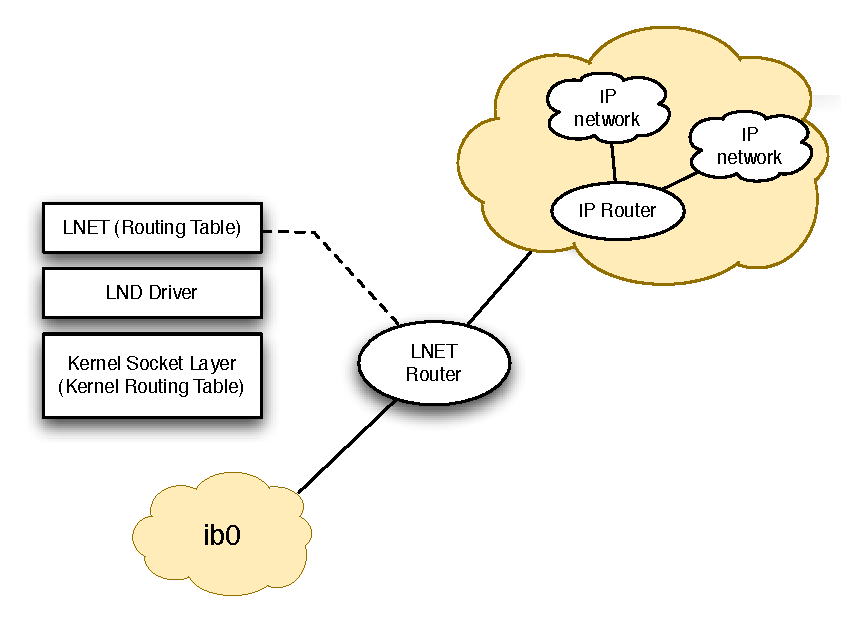
\includegraphics[width=4.5in]{img/lnet_topology}
\label{fig:lnet_topology}
\caption{Illustration of LNET routing layer stack.}
\end{figure}


\subsubsection{Asymmetric Routing Failure}

This topic highlights a deficit we discovered in the current LNET production code. It is
pertinent to the general discussion on LNET, and
we believe it would be good to share our observation with a broader audience. The problem is
that it can be difficult for a router to reliably determine if an interface is
down. Right now, LNET does not even try to do it. So for a configuration
where a router has two interfaces, such as \url{tcp0} and \url{ib0}, if the \url{ib0}
interface is down and end nodes connected with \url{tcp0} are still pushing
data, this will result in an intermittent communication failure.

One idea towards solving this problem is that the  LNET router can try to
detect the transmission problem, then temporally disable all its interfaces. A
router might be able to do this more intelligently by disabling only some
interfaces if it has information on the full topology and the incoming path
that clients use. Until then, shutting down all of its interfaces seems to be
better than suffering timeout as a result of intermittent communication
failure.

\subsubsection{Routing Buffer Management and Flow Control}

Upon initialization, an LNET router pre-allocates a fixed number of routing
buffers. The LNET layer of an end node won't need to do this (except when
initializing its routing tables). Allocating and managing routing buffers are
the primary, if not the only, difference between the execution logic of an end
node and a router.

As routing buffers are limited resources, to prevent a single end node from
overwhelming a router, each end node is given a quota. Once a buffer has been
forwarded, it can be recycled again. The quota for each end node is also known
as \textbf{buffer credit}. It is only significant for routers, and it is
different from the ``RPCs in flight" credit, which is known as \textbf{peer to
peer credit}. One RPC can involve several LNET messages (at most ten), and these
can be one request LNET message, one reply LNET message, and in the case of a
bulk transfer, there could be four LNET messages going one way, and four LNET
messages going in the opposite direction. This also implies that the bulk
transfer LNET messages are part of the bulk RPC transaction, but they are
\textbf{not} considered an RPC. Therefore, they (the four bulk transfer messages)
are not counted towards RPCs in flight.

There are three kinds of router buffers: 1MB (maximum amount of payload an LNET
message can carry), 4KB for small messages, and zero payload buffers for tiny
messages such as ACK. 

Requests from an end node are on a first come, first served basis. If requests from
a particular end node exceed its quota, then its next request will not be
handled until the router buffer is freed, which is essentially the way LNET
layer does flow control (flow control is point-to-point). It is up to the upper
layer to implement an end-to-end flow control, for example, by number of RPCs
in flight. The buffer can be freed when the underlying LND calls the
\url{lnet_finalize()} as an indication that LND considers the forwarding done,
but it doesn't really mean the message has been put on the wire. Depending on
the size of the message, LND and kernel may have different logics for handling
it. The only requirement from LNET is, once \url{lnet_finalize()} is invoked,
LNET should be able to recycle the buffer freely. 

Logically, LNET has a single queue, and incoming messages from all interfaces
are queued and processed in order. Each interface has its own interface
queues; however, that is not a concern of LNET since this is interrupt-driven.
So it is guaranteed that each incoming message is handled in the order it
arrives.  


\subsubsection{Fine Grain Routing}

This feature is a recent development (Lustre bug \#15332) for Jaguar/Spider
deployment at ORNL. The motivation is that LNET doesn't assign weights to
routes. So if you have multiple routers that reach the same destination,
LNET will perform a round robin algorithm to distribute the load, and this
applies to both end node and router. What fine grained routing adds, is simply,
to assign weights to different routers, preconfigured by the system
administrator.  The goal is that \textit{better} routes gets more traffic.
Here, better is defined by the site system administrator.

\begin{Verbatim}
   dest network 1:
        w1    (router 1, router 3)
        w2    (router 4, router 5)
        w3    (router 2)
\end{Verbatim}

So for example, you can specify different weight classes and assign routers to
each to indicate your preference. If $w_1 < w_2$, then $w_1$ is the preferred
weight class of the two. Within a given weight class, routers are equal.

More specific to our case, this mechanism provides the potential for a client
to pick a router closer to its proximity as its preferred router.
